\chapter{Verification}

\section{Instruction decoding}
This sub-unit was tested along with the rest of the pipeline, since several signals coming from other stages are important to determine the control flow. For instance, the misprediction flag is generated in the MEM stage and the data used by the hazard detection unit comes from the pipeline registers. The instruction decoding stage was connected to a behavioral ALU in order to focus the debugging effort on the instruction sequence. \autoref{fig:wave} shows the occurrence of a branch (at $t=1.2\, \mu$s), the corresponding jump due to the taken prediction and the subsequent recovery two clock cycles later, when the prediction is found to be incorrect.

\begin{figure}
	\makebox[\textwidth][c]{
	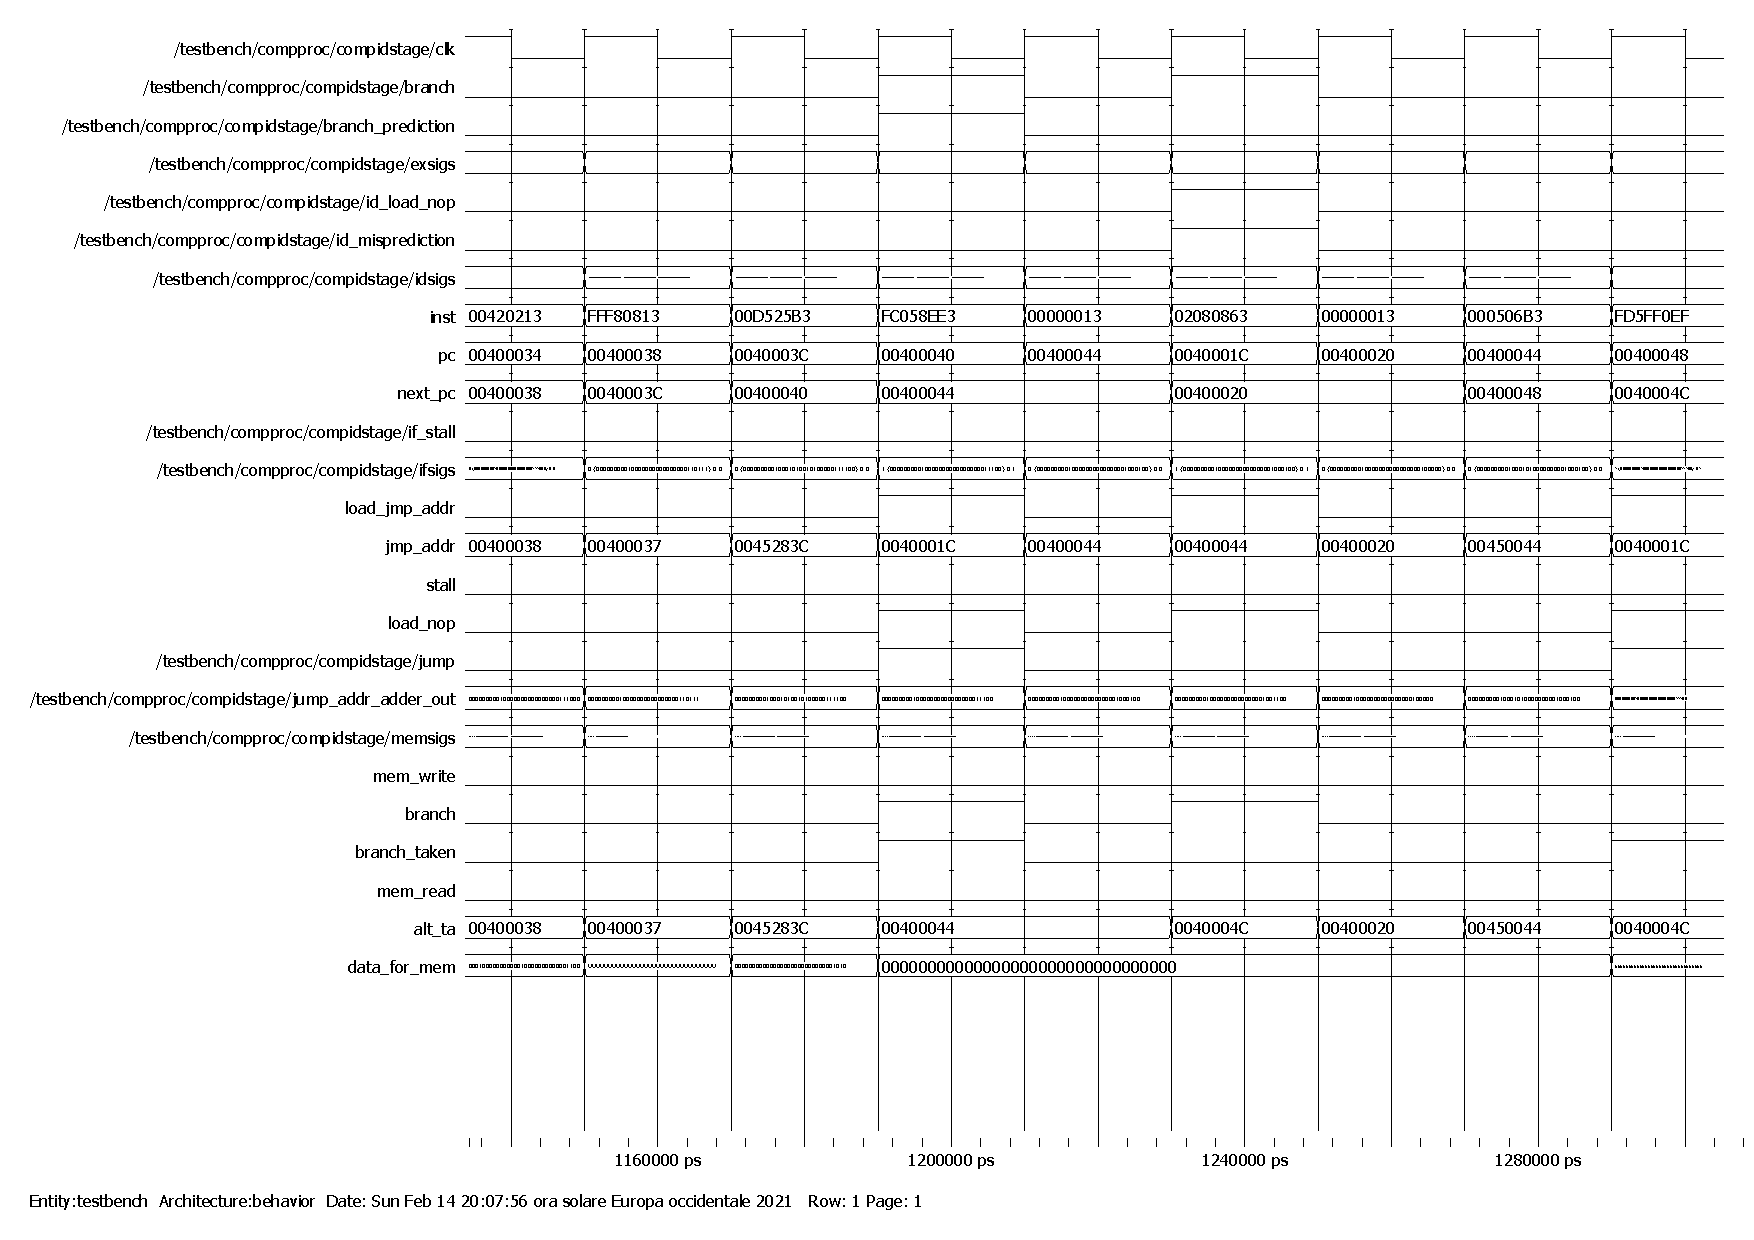
\includegraphics[angle=90, width=1.2\textwidth]{./images/wave.pdf}}
	\caption{Instruction decoding stage signals showing the occurrence of a branch and the following flush due to its misprediction.}
	\label{fig:wave}
\end{figure}